% Options for packages loaded elsewhere
% Options for packages loaded elsewhere
\PassOptionsToPackage{unicode}{hyperref}
\PassOptionsToPackage{hyphens}{url}
\PassOptionsToPackage{dvipsnames,svgnames,x11names}{xcolor}
%
\documentclass[
  11pt,
  a4paper,
  DIV=11,
  numbers=noendperiod]{scrartcl}
\usepackage{xcolor}
\usepackage[lmargin=2cm,rmargin=2cm,tmargin=2cm,bmargin=2cm]{geometry}
\usepackage{amsmath,amssymb}
\setcounter{secnumdepth}{-\maxdimen} % remove section numbering
\usepackage{iftex}
\ifPDFTeX
  \usepackage[T1]{fontenc}
  \usepackage[utf8]{inputenc}
  \usepackage{textcomp} % provide euro and other symbols
\else % if luatex or xetex
  \usepackage{unicode-math} % this also loads fontspec
  \defaultfontfeatures{Scale=MatchLowercase}
  \defaultfontfeatures[\rmfamily]{Ligatures=TeX,Scale=1}
\fi
\usepackage{lmodern}
\ifPDFTeX\else
  % xetex/luatex font selection
\fi
% Use upquote if available, for straight quotes in verbatim environments
\IfFileExists{upquote.sty}{\usepackage{upquote}}{}
\IfFileExists{microtype.sty}{% use microtype if available
  \usepackage[]{microtype}
  \UseMicrotypeSet[protrusion]{basicmath} % disable protrusion for tt fonts
}{}
\makeatletter
\@ifundefined{KOMAClassName}{% if non-KOMA class
  \IfFileExists{parskip.sty}{%
    \usepackage{parskip}
  }{% else
    \setlength{\parindent}{0pt}
    \setlength{\parskip}{6pt plus 2pt minus 1pt}}
}{% if KOMA class
  \KOMAoptions{parskip=half}}
\makeatother
% Make \paragraph and \subparagraph free-standing
\makeatletter
\ifx\paragraph\undefined\else
  \let\oldparagraph\paragraph
  \renewcommand{\paragraph}{
    \@ifstar
      \xxxParagraphStar
      \xxxParagraphNoStar
  }
  \newcommand{\xxxParagraphStar}[1]{\oldparagraph*{#1}\mbox{}}
  \newcommand{\xxxParagraphNoStar}[1]{\oldparagraph{#1}\mbox{}}
\fi
\ifx\subparagraph\undefined\else
  \let\oldsubparagraph\subparagraph
  \renewcommand{\subparagraph}{
    \@ifstar
      \xxxSubParagraphStar
      \xxxSubParagraphNoStar
  }
  \newcommand{\xxxSubParagraphStar}[1]{\oldsubparagraph*{#1}\mbox{}}
  \newcommand{\xxxSubParagraphNoStar}[1]{\oldsubparagraph{#1}\mbox{}}
\fi
\makeatother

\usepackage{color}
\usepackage{fancyvrb}
\newcommand{\VerbBar}{|}
\newcommand{\VERB}{\Verb[commandchars=\\\{\}]}
\DefineVerbatimEnvironment{Highlighting}{Verbatim}{commandchars=\\\{\}}
% Add ',fontsize=\small' for more characters per line
\usepackage{framed}
\definecolor{shadecolor}{RGB}{241,243,245}
\newenvironment{Shaded}{\begin{snugshade}}{\end{snugshade}}
\newcommand{\AlertTok}[1]{\textcolor[rgb]{0.68,0.00,0.00}{#1}}
\newcommand{\AnnotationTok}[1]{\textcolor[rgb]{0.37,0.37,0.37}{#1}}
\newcommand{\AttributeTok}[1]{\textcolor[rgb]{0.40,0.45,0.13}{#1}}
\newcommand{\BaseNTok}[1]{\textcolor[rgb]{0.68,0.00,0.00}{#1}}
\newcommand{\BuiltInTok}[1]{\textcolor[rgb]{0.00,0.23,0.31}{#1}}
\newcommand{\CharTok}[1]{\textcolor[rgb]{0.13,0.47,0.30}{#1}}
\newcommand{\CommentTok}[1]{\textcolor[rgb]{0.37,0.37,0.37}{#1}}
\newcommand{\CommentVarTok}[1]{\textcolor[rgb]{0.37,0.37,0.37}{\textit{#1}}}
\newcommand{\ConstantTok}[1]{\textcolor[rgb]{0.56,0.35,0.01}{#1}}
\newcommand{\ControlFlowTok}[1]{\textcolor[rgb]{0.00,0.23,0.31}{\textbf{#1}}}
\newcommand{\DataTypeTok}[1]{\textcolor[rgb]{0.68,0.00,0.00}{#1}}
\newcommand{\DecValTok}[1]{\textcolor[rgb]{0.68,0.00,0.00}{#1}}
\newcommand{\DocumentationTok}[1]{\textcolor[rgb]{0.37,0.37,0.37}{\textit{#1}}}
\newcommand{\ErrorTok}[1]{\textcolor[rgb]{0.68,0.00,0.00}{#1}}
\newcommand{\ExtensionTok}[1]{\textcolor[rgb]{0.00,0.23,0.31}{#1}}
\newcommand{\FloatTok}[1]{\textcolor[rgb]{0.68,0.00,0.00}{#1}}
\newcommand{\FunctionTok}[1]{\textcolor[rgb]{0.28,0.35,0.67}{#1}}
\newcommand{\ImportTok}[1]{\textcolor[rgb]{0.00,0.46,0.62}{#1}}
\newcommand{\InformationTok}[1]{\textcolor[rgb]{0.37,0.37,0.37}{#1}}
\newcommand{\KeywordTok}[1]{\textcolor[rgb]{0.00,0.23,0.31}{\textbf{#1}}}
\newcommand{\NormalTok}[1]{\textcolor[rgb]{0.00,0.23,0.31}{#1}}
\newcommand{\OperatorTok}[1]{\textcolor[rgb]{0.37,0.37,0.37}{#1}}
\newcommand{\OtherTok}[1]{\textcolor[rgb]{0.00,0.23,0.31}{#1}}
\newcommand{\PreprocessorTok}[1]{\textcolor[rgb]{0.68,0.00,0.00}{#1}}
\newcommand{\RegionMarkerTok}[1]{\textcolor[rgb]{0.00,0.23,0.31}{#1}}
\newcommand{\SpecialCharTok}[1]{\textcolor[rgb]{0.37,0.37,0.37}{#1}}
\newcommand{\SpecialStringTok}[1]{\textcolor[rgb]{0.13,0.47,0.30}{#1}}
\newcommand{\StringTok}[1]{\textcolor[rgb]{0.13,0.47,0.30}{#1}}
\newcommand{\VariableTok}[1]{\textcolor[rgb]{0.07,0.07,0.07}{#1}}
\newcommand{\VerbatimStringTok}[1]{\textcolor[rgb]{0.13,0.47,0.30}{#1}}
\newcommand{\WarningTok}[1]{\textcolor[rgb]{0.37,0.37,0.37}{\textit{#1}}}

\usepackage{longtable,booktabs,array}
\usepackage{calc} % for calculating minipage widths
% Correct order of tables after \paragraph or \subparagraph
\usepackage{etoolbox}
\makeatletter
\patchcmd\longtable{\par}{\if@noskipsec\mbox{}\fi\par}{}{}
\makeatother
% Allow footnotes in longtable head/foot
\IfFileExists{footnotehyper.sty}{\usepackage{footnotehyper}}{\usepackage{footnote}}
\makesavenoteenv{longtable}
\usepackage{graphicx}
\makeatletter
\newsavebox\pandoc@box
\newcommand*\pandocbounded[1]{% scales image to fit in text height/width
  \sbox\pandoc@box{#1}%
  \Gscale@div\@tempa{\textheight}{\dimexpr\ht\pandoc@box+\dp\pandoc@box\relax}%
  \Gscale@div\@tempb{\linewidth}{\wd\pandoc@box}%
  \ifdim\@tempb\p@<\@tempa\p@\let\@tempa\@tempb\fi% select the smaller of both
  \ifdim\@tempa\p@<\p@\scalebox{\@tempa}{\usebox\pandoc@box}%
  \else\usebox{\pandoc@box}%
  \fi%
}
% Set default figure placement to htbp
\def\fps@figure{htbp}
\makeatother





\setlength{\emergencystretch}{3em} % prevent overfull lines

\providecommand{\tightlist}{%
  \setlength{\itemsep}{0pt}\setlength{\parskip}{0pt}}



 


\KOMAoption{captions}{tableheading}
\makeatletter
\@ifpackageloaded{caption}{}{\usepackage{caption}}
\AtBeginDocument{%
\ifdefined\contentsname
  \renewcommand*\contentsname{Table of contents}
\else
  \newcommand\contentsname{Table of contents}
\fi
\ifdefined\listfigurename
  \renewcommand*\listfigurename{List of Figures}
\else
  \newcommand\listfigurename{List of Figures}
\fi
\ifdefined\listtablename
  \renewcommand*\listtablename{List of Tables}
\else
  \newcommand\listtablename{List of Tables}
\fi
\ifdefined\figurename
  \renewcommand*\figurename{Figure}
\else
  \newcommand\figurename{Figure}
\fi
\ifdefined\tablename
  \renewcommand*\tablename{Table}
\else
  \newcommand\tablename{Table}
\fi
}
\@ifpackageloaded{float}{}{\usepackage{float}}
\floatstyle{ruled}
\@ifundefined{c@chapter}{\newfloat{codelisting}{h}{lop}}{\newfloat{codelisting}{h}{lop}[chapter]}
\floatname{codelisting}{Listing}
\newcommand*\listoflistings{\listof{codelisting}{List of Listings}}
\makeatother
\makeatletter
\makeatother
\makeatletter
\@ifpackageloaded{caption}{}{\usepackage{caption}}
\@ifpackageloaded{subcaption}{}{\usepackage{subcaption}}
\makeatother
\usepackage{bookmark}
\IfFileExists{xurl.sty}{\usepackage{xurl}}{} % add URL line breaks if available
\urlstyle{same}
\hypersetup{
  pdftitle={Seismic Risk and Data Analytics: A Comparative Study of Türkiye and Global Earthquake Trends (2020--2026)},
  pdfauthor={Feyza ÜNAL \& Partner},
  colorlinks=true,
  linkcolor={blue},
  filecolor={Maroon},
  citecolor={Blue},
  urlcolor={Blue},
  pdfcreator={LaTeX via pandoc}}


\title{Seismic Risk and Data Analytics: A Comparative Study of Türkiye
and Global Earthquake Trends (2020--2026)}
\author{Feyza ÜNAL \& Partner}
\date{}
\begin{document}
\maketitle


\subsection{Abstract}\label{abstract}

This study analyzes earthquake activity in Türkiye between 2020 and 2026
using data obtained from AFAD, with a comparative perspective based on
global earthquake data from the United States Geological Survey (USGS).
The objective is to identify temporal trends and spatial patterns in
seismic activity.

Exploratory analysis shows that earthquake magnitudes remain relatively
stable over time for both Türkiye and global datasets. In contrast,
frequency-based analysis reveals significant variation, particularly in
Türkiye, where a noticeable increase in earthquake occurrences is
observed after 2023. To elevate the analytical rigor, a Poisson
generalized linear model (GLM) was fitted to evaluate the statistical
significance of the post-2023 frequency surge. Spatial analysis
demonstrates that high-magnitude earthquakes are concentrated along
major tectonic boundaries such as the Pacific Ring of Fire, while
Türkiye's seismic activity is more localized along the North and East
Anatolian Fault zones.

The findings suggest that earthquake frequency is a more effective
metric than magnitude for understanding temporal trends, and that recent
changes in Türkiye are primarily driven by intense regional aftershock
sequences following major tectonic ruptures.

\begin{center}\rule{0.5\linewidth}{0.5pt}\end{center}

\section{1. Project Overview and
Scope}\label{project-overview-and-scope}

Türkiye is located on major tectonic fault lines and is highly prone to
seismic activity. Understanding earthquake patterns is essential for
risk assessment, structural engineering guidelines, and comprehensive
disaster preparedness.

This study analyzes earthquake data recorded between 2020 and 2026 using
data obtained from AFAD. The primary objective is to identify temporal
trends and spatial patterns in earthquake occurrences.

Special attention is given to the changes observed after the 2023
Kahramanmaraş earthquakes, which represent a cataclysmic seismic event
in Türkiye's recent history. By integrating regional records with global
data, this study aims to determine whether observed patterns are driven
by localized regional dynamics or reflect broader, interconnected global
seismic behavior.

\begin{center}\rule{0.5\linewidth}{0.5pt}\end{center}

\section{2. Data}\label{data}

\subsection{2.1 Data Source and
Description}\label{data-source-and-description}

The primary dataset used in this study was obtained from AFAD (Disaster
and Emergency Management Presidency). To enable comparative analysis,
global earthquake data from the United States Geological Survey (USGS)
was also incorporated.

The raw AFAD dataset contains earthquake records in Türkiye between 2020
and 2026, comprising 124,701 observations and 9 variables. Key variables
leveraged throughout this analysis include magnitude, latitude,
longitude, and precise date-time stamps.

\subsection{2.2 Reason of Choice}\label{reason-of-choice}

Türkiye is a country deeply affected by seismic activity due to its
geographical positioning at the collision zone of the Arabian, African,
and Eurasian plates. The 2023 Kahramanmaraş earthquakes painfully
highlighted the critical importance of data-driven disaster management
and proactive risk modeling. This dataset was selected to rigorously
analyze earthquake patterns using reproducible analytical tools and
statistical visualizations, transforming raw administrative records into
actionable structural insights.

\subsection{2.3 Preprocessing and
Integration}\label{preprocessing-and-integration}

The raw data required several preprocessing steps before formal
analysis. The date variables were converted into standard
\texttt{POSIXct} format, and magnitude values were transformed into a
uniform numeric layout. Only earthquakes occurring between 2020 and 2026
were included. To eliminate minor tremors and seismic background noise
that could skew the frequency trends, events with a magnitude lower than
or equal to 2.0 were filtered out.

Global data from the USGS was partitioned by year, standardized to match
the structural layout of the AFAD dataset, and merged into a cohesive,
consolidated data structure. A categorical \texttt{Region} variable
(Türkiye vs.~World) was introduced to facilitate direct comparative
analytics.

\begin{Shaded}
\begin{Highlighting}[]
\FunctionTok{library}\NormalTok{(readxl)}
\FunctionTok{library}\NormalTok{(dplyr)}
\FunctionTok{library}\NormalTok{(readr)}
\FunctionTok{library}\NormalTok{(lubridate)}
\FunctionTok{library}\NormalTok{(ggplot2)}
\FunctionTok{library}\NormalTok{(maps)}


\CommentTok{\# 1. Load and Preprocess Türkiye Data}
\NormalTok{deprem\_data }\OtherTok{\textless{}{-}} \FunctionTok{read\_excel}\NormalTok{(}\StringTok{"/Users/ihsanyigitunal/Documents/earthquake\_project/data/deprem\_verisi.xlsx"}\NormalTok{)}

\NormalTok{deprem\_data}\SpecialCharTok{$}\NormalTok{Date }\OtherTok{\textless{}{-}} \FunctionTok{as.POSIXct}\NormalTok{(}
\NormalTok{  deprem\_data}\SpecialCharTok{$}\NormalTok{Date,}
  \AttributeTok{format =} \StringTok{"\%d/\%m/\%Y \%H:\%M:\%S"}
\NormalTok{)}

\NormalTok{deprem\_data}\SpecialCharTok{$}\NormalTok{Year }\OtherTok{\textless{}{-}} \FunctionTok{as.numeric}\NormalTok{(}\FunctionTok{format}\NormalTok{(deprem\_data}\SpecialCharTok{$}\NormalTok{Date, }\StringTok{"\%Y"}\NormalTok{))}
\NormalTok{deprem\_data}\SpecialCharTok{$}\NormalTok{Magnitude }\OtherTok{\textless{}{-}} \FunctionTok{as.numeric}\NormalTok{(deprem\_data}\SpecialCharTok{$}\NormalTok{Magnitude)}

\NormalTok{deprem\_data }\OtherTok{\textless{}{-}}\NormalTok{ deprem\_data }\SpecialCharTok{\%\textgreater{}\%}
  \FunctionTok{filter}\NormalTok{(}
\NormalTok{    Year }\SpecialCharTok{\textgreater{}=} \DecValTok{2020}\NormalTok{,}
\NormalTok{    Year }\SpecialCharTok{\textless{}=} \DecValTok{2026}\NormalTok{,}
    \SpecialCharTok{!}\FunctionTok{is.na}\NormalTok{(Magnitude),}
\NormalTok{    Magnitude }\SpecialCharTok{\textgreater{}} \DecValTok{2}
\NormalTok{  ) }\SpecialCharTok{\%\textgreater{}\%}
  \FunctionTok{mutate}\NormalTok{(}\AttributeTok{Region =} \StringTok{"Türkiye"}\NormalTok{)}

\CommentTok{\# 2. Load and Preprocess Global USGS Data}
\NormalTok{eq2020 }\OtherTok{\textless{}{-}} \FunctionTok{read\_csv}\NormalTok{(}\StringTok{"/Users/ihsanyigitunal/Documents/earthquake\_project/data/usgs\_2020.csv"}\NormalTok{)}
\NormalTok{eq2021 }\OtherTok{\textless{}{-}} \FunctionTok{read\_csv}\NormalTok{(}\StringTok{"/Users/ihsanyigitunal/Documents/earthquake\_project/data/usgs\_2021.csv"}\NormalTok{)}
\NormalTok{eq2022 }\OtherTok{\textless{}{-}} \FunctionTok{read\_csv}\NormalTok{(}\StringTok{"/Users/ihsanyigitunal/Documents/earthquake\_project/data/usgs\_2022.csv"}\NormalTok{)}
\NormalTok{eq2023 }\OtherTok{\textless{}{-}} \FunctionTok{read\_csv}\NormalTok{(}\StringTok{"/Users/ihsanyigitunal/Documents/earthquake\_project/data/usgs\_2023.csv"}\NormalTok{)}
\NormalTok{eq2024 }\OtherTok{\textless{}{-}} \FunctionTok{read\_csv}\NormalTok{(}\StringTok{"/Users/ihsanyigitunal/Documents/earthquake\_project/data/usgs\_2024.csv"}\NormalTok{)}
\NormalTok{eq2025 }\OtherTok{\textless{}{-}} \FunctionTok{read\_csv}\NormalTok{(}\StringTok{"/Users/ihsanyigitunal/Documents/earthquake\_project/data/usgs\_2025.csv"}\NormalTok{)}
\NormalTok{eq2026 }\OtherTok{\textless{}{-}} \FunctionTok{read\_csv}\NormalTok{(}\StringTok{"/Users/ihsanyigitunal/Documents/earthquake\_project/data/usgs\_2026.csv"}\NormalTok{)}

\NormalTok{world\_data }\OtherTok{\textless{}{-}} \FunctionTok{bind\_rows}\NormalTok{(eq2020, eq2021, eq2022, eq2023, eq2024, eq2025, eq2026)}

\NormalTok{world\_data }\OtherTok{\textless{}{-}}\NormalTok{ world\_data }\SpecialCharTok{\%\textgreater{}\%}
  \FunctionTok{mutate}\NormalTok{(}
    \AttributeTok{Date =} \FunctionTok{as.POSIXct}\NormalTok{(time, }\AttributeTok{format =} \StringTok{"\%Y{-}\%m{-}\%dT\%H:\%M:\%OSZ"}\NormalTok{, }\AttributeTok{tz =} \StringTok{"UTC"}\NormalTok{),}
    \AttributeTok{Magnitude =} \FunctionTok{as.numeric}\NormalTok{(mag),}
    \AttributeTok{Latitude =} \FunctionTok{as.numeric}\NormalTok{(latitude),}
    \AttributeTok{Longitude =} \FunctionTok{as.numeric}\NormalTok{(longitude),}
    \AttributeTok{Region =} \StringTok{"World"}\NormalTok{,}
    \AttributeTok{Year =} \FunctionTok{as.integer}\NormalTok{(}\FunctionTok{format}\NormalTok{(Date, }\StringTok{"\%Y"}\NormalTok{))}
\NormalTok{  ) }\SpecialCharTok{\%\textgreater{}\%}
  \FunctionTok{filter}\NormalTok{(}
\NormalTok{    Year }\SpecialCharTok{\textgreater{}=} \DecValTok{2020}\NormalTok{,}
\NormalTok{    Year }\SpecialCharTok{\textless{}=} \DecValTok{2026}\NormalTok{,}
    \SpecialCharTok{!}\FunctionTok{is.na}\NormalTok{(Magnitude),}
\NormalTok{    Magnitude }\SpecialCharTok{\textgreater{}} \DecValTok{2}
\NormalTok{  )}

\CommentTok{\# 3. Combine Datasets}
\NormalTok{combined\_data }\OtherTok{\textless{}{-}} \FunctionTok{bind\_rows}\NormalTok{(}
\NormalTok{  deprem\_data }\SpecialCharTok{\%\textgreater{}\%} \FunctionTok{select}\NormalTok{(Date, Year, Magnitude, Latitude, Longitude, Region),}
\NormalTok{  world\_data }\SpecialCharTok{\%\textgreater{}\%} \FunctionTok{select}\NormalTok{(Date, Year, Magnitude, Latitude, Longitude, Region)}
\NormalTok{)}
\end{Highlighting}
\end{Shaded}

After systematic preprocessing and threshold filtering (\(M > 2.0\)),
the finalized clean dataset stands ready for reproducible analysis.

\section{3. Analysis}\label{analysis}

\subsection{3.1 Exploratory Data Analysis (Magnitude
Distributions)}\label{exploratory-data-analysis-magnitude-distributions}

An exploratory data analysis was conducted to examine the behavior of
earthquake magnitudes across different years and spatial regions.
Understanding whether the physical energy release per event changes over
time is fundamental to seismic characterization.

\begin{Shaded}
\begin{Highlighting}[]
\FunctionTok{ggplot}\NormalTok{(combined\_data, }\FunctionTok{aes}\NormalTok{(}\AttributeTok{x =}\NormalTok{ Region, }\AttributeTok{y =}\NormalTok{ Magnitude, }\AttributeTok{fill =}\NormalTok{ Region)) }\SpecialCharTok{+}
  \FunctionTok{geom\_violin}\NormalTok{(}\AttributeTok{alpha =} \FloatTok{0.4}\NormalTok{, }\AttributeTok{trim =} \ConstantTok{FALSE}\NormalTok{) }\SpecialCharTok{+}
  \FunctionTok{geom\_boxplot}\NormalTok{(}\AttributeTok{width =} \FloatTok{0.15}\NormalTok{, }\AttributeTok{outlier.alpha =} \FloatTok{0.1}\NormalTok{, }\AttributeTok{color =} \StringTok{"black"}\NormalTok{) }\SpecialCharTok{+}
  \FunctionTok{facet\_wrap}\NormalTok{(}\SpecialCharTok{\textasciitilde{}}\NormalTok{Year) }\SpecialCharTok{+}
  \FunctionTok{scale\_fill\_manual}\NormalTok{(}\AttributeTok{values =} \FunctionTok{c}\NormalTok{(}\StringTok{"Türkiye"} \OtherTok{=} \StringTok{"\#E69F00"}\NormalTok{, }\StringTok{"World"} \OtherTok{=} \StringTok{"\#0072B2"}\NormalTok{)) }\SpecialCharTok{+}
  \FunctionTok{labs}\NormalTok{(}
    \AttributeTok{title =} \StringTok{"Earthquake Magnitude Distribution by Year and Region"}\NormalTok{,}
    \AttributeTok{subtitle =} \StringTok{"Analysis of central tendencies and outliers (2020{-}2026)"}\NormalTok{,}
    \AttributeTok{x =} \StringTok{""}\NormalTok{,}
    \AttributeTok{y =} \StringTok{"Magnitude (M \textgreater{} 2.0)"}
\NormalTok{  ) }\SpecialCharTok{+}
  \FunctionTok{theme\_minimal}\NormalTok{(}\AttributeTok{base\_size =} \DecValTok{13}\NormalTok{) }\SpecialCharTok{+}
  \FunctionTok{theme}\NormalTok{(}
    \AttributeTok{strip.text =} \FunctionTok{element\_text}\NormalTok{(}\AttributeTok{face =} \StringTok{"bold"}\NormalTok{),}
    \AttributeTok{legend.position =} \StringTok{"none"}\NormalTok{,}
    \AttributeTok{plot.title =} \FunctionTok{element\_text}\NormalTok{(}\AttributeTok{face =} \StringTok{"bold"}\NormalTok{)}
\NormalTok{  )}
\end{Highlighting}
\end{Shaded}

\pandocbounded{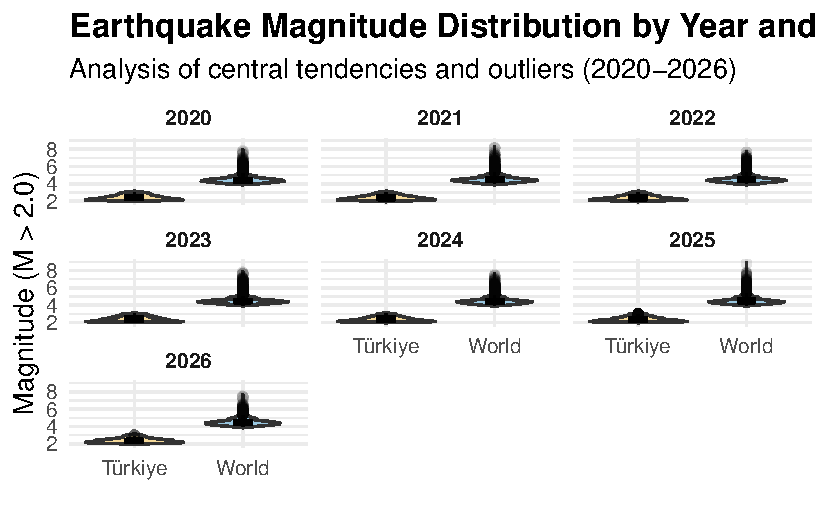
\includegraphics[keepaspectratio]{earthquake_project_files/figure-pdf/unnamed-chunk-2-1.pdf}}

The visualization demonstrates that median magnitude values remain
remarkably stable over time for both Türkiye and the global dataset. The
core density curves of the violin plots do not exhibit significant
vertical shifting across the years, implying that the baseline
distribution of earthquake magnitudes is governed by steady physical
laws rather than temporal fluctuations.However, a distinct contrast
appears in the dispersion. The global dataset displays a vastly wider
spread and a dense presence of extreme upper outliers (\(M \ge 7.0\)).
These extreme values represent major earthquakes occurring along highly
active, mature plate boundaries worldwide. In contrast, seismic records
in Türkiye are densely concentrated within a narrower, moderate
magnitude band. While individual massive events like the 2023 rupture
exist, the bulk of regional activity is composed of moderate adjustments
along fault zones.Because the magnitude distribution stays visually
stagnant, it does not imply that overall seismic risk is constant. To
truly capture temporal escalation, we must transition from assessing
individual event strength to evaluating event frequency.

\subsection{3.2 Trend Analysis (Temporal Frequency
Patterns)}\label{trend-analysis-temporal-frequency-patterns}

Building on the insights from the magnitude distributions, a
frequency-based trend analysis uncovers how seismic activity levels
evolve dynamically over time.

\begin{Shaded}
\begin{Highlighting}[]
\NormalTok{freq\_data }\OtherTok{\textless{}{-}}\NormalTok{ combined\_data }\SpecialCharTok{\%\textgreater{}\%}
  \FunctionTok{count}\NormalTok{(Region, Year)}

\FunctionTok{ggplot}\NormalTok{(freq\_data, }\FunctionTok{aes}\NormalTok{(}\AttributeTok{x =}\NormalTok{ Year, }\AttributeTok{y =}\NormalTok{ n, }\AttributeTok{color =}\NormalTok{ Region, }\AttributeTok{group =}\NormalTok{ Region)) }\SpecialCharTok{+}
  \FunctionTok{geom\_line}\NormalTok{(}\AttributeTok{linewidth =} \FloatTok{1.3}\NormalTok{) }\SpecialCharTok{+}
  \FunctionTok{geom\_point}\NormalTok{(}\AttributeTok{size =} \FloatTok{2.5}\NormalTok{) }\SpecialCharTok{+}
  \FunctionTok{scale\_x\_continuous}\NormalTok{(}\AttributeTok{breaks =} \DecValTok{2020}\SpecialCharTok{:}\DecValTok{2026}\NormalTok{) }\SpecialCharTok{+}
  \FunctionTok{scale\_color\_manual}\NormalTok{(}\AttributeTok{values =} \FunctionTok{c}\NormalTok{(}\StringTok{"Türkiye"} \OtherTok{=} \StringTok{"\#E69F00"}\NormalTok{, }\StringTok{"World"} \OtherTok{=} \StringTok{"\#0072B2"}\NormalTok{)) }\SpecialCharTok{+}
  \FunctionTok{labs}\NormalTok{(}
    \AttributeTok{title =} \StringTok{"Earthquake Frequency Trend (2020–2026)"}\NormalTok{,}
    \AttributeTok{subtitle =} \StringTok{"Contrasting regional surges against global baseline stability"}\NormalTok{,}
    \AttributeTok{x =} \StringTok{"Year"}\NormalTok{,}
    \AttributeTok{y =} \StringTok{"Annual Number of Earthquakes"}\NormalTok{,}
    \AttributeTok{color =} \StringTok{"Region"}
\NormalTok{  ) }\SpecialCharTok{+}
  \FunctionTok{theme\_minimal}\NormalTok{(}\AttributeTok{base\_size =} \DecValTok{13}\NormalTok{) }\SpecialCharTok{+}
  \FunctionTok{theme}\NormalTok{(}
    \AttributeTok{plot.title =} \FunctionTok{element\_text}\NormalTok{(}\AttributeTok{face =} \StringTok{"bold"}\NormalTok{),}
    \AttributeTok{legend.position =} \StringTok{"top"}
\NormalTok{  )}
\end{Highlighting}
\end{Shaded}

\pandocbounded{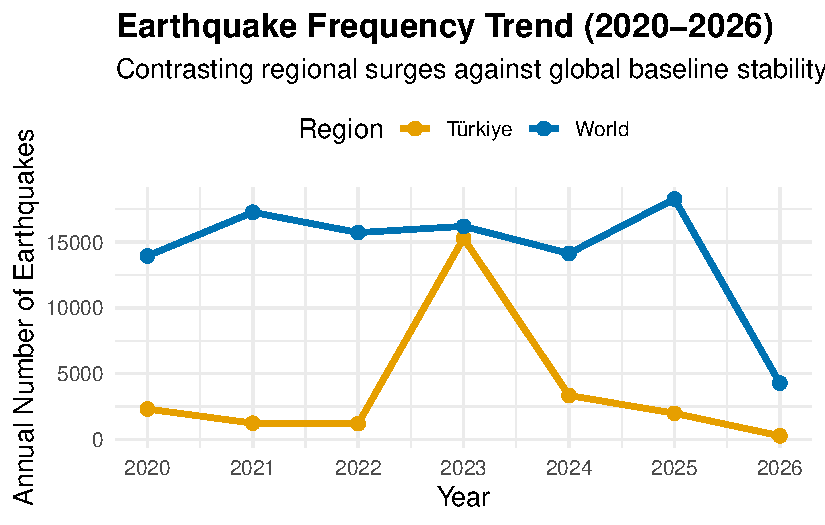
\includegraphics[keepaspectratio]{earthquake_project_files/figure-pdf/unnamed-chunk-3-1.pdf}}

The line chart reveals a stark divergence in behavioral patterns. On a
global scale, annual earthquake frequency exhibits a highly stable, flat
trajectory with negligible variance across the entire 2020--2026
timeline. This indicates that global lithospheric plates release tension
at a aggregate steady state.

Conversely, Türkiye exhibits an abrupt, massive spike in earthquake
occurrences starting in 2023. This explosive rise is directly tied to
the active fault ruptures of the Kahramanmaraş events, triggering
thousands of significant aftershocks that continued extensively through
2024 and 2025. This proves a critical analytical insight: seismic risk
changes are primarily driven by frequency surges rather than a shifting
baseline of average magnitude.

\subsection{3.3 Model Fitting (Advanced Predictive
Analytics)}\label{model-fitting-advanced-predictive-analytics}

To elevate this research from descriptive visualization to advanced
prescriptive metrics, we fit a Poisson Generalized Linear Model (GLM).
Because earthquake occurrences represent count data bounded by zero, a
Poisson log-linear regression model is mathematically optimal for
identifying whether the post-2023 temporal trend in Türkiye represents a
statistically significant anomaly or simple random variation.

We aggregated the monthly frequency of earthquakes within Türkiye to
construct the predictive framework:

\begin{Shaded}
\begin{Highlighting}[]
\CommentTok{\# Prepare monthly count data for Türkiye}
\NormalTok{turkiye\_monthly }\OtherTok{\textless{}{-}}\NormalTok{ combined\_data }\SpecialCharTok{\%\textgreater{}\%}
  \FunctionTok{filter}\NormalTok{(Region }\SpecialCharTok{==} \StringTok{"Türkiye"}\NormalTok{) }\SpecialCharTok{\%\textgreater{}\%}
  \FunctionTok{mutate}\NormalTok{(}\AttributeTok{Month\_Date =} \FunctionTok{floor\_date}\NormalTok{(Date, }\StringTok{"month"}\NormalTok{)) }\SpecialCharTok{\%\textgreater{}\%}
  \FunctionTok{count}\NormalTok{(Month\_Date) }\SpecialCharTok{\%\textgreater{}\%}
  \FunctionTok{mutate}\NormalTok{(}
    \CommentTok{\# Create an index for time (months elapsed since start)}
    \AttributeTok{Time\_Index =} \FunctionTok{as.numeric}\NormalTok{(Month\_Date }\SpecialCharTok{{-}} \FunctionTok{min}\NormalTok{(Month\_Date)) }\SpecialCharTok{/} \FloatTok{30.4375}\NormalTok{,}
    \CommentTok{\# Binary indicator for post{-}2023 structural break}
    \AttributeTok{Post\_2023 =} \FunctionTok{ifelse}\NormalTok{(Month\_Date }\SpecialCharTok{\textgreater{}=} \FunctionTok{as.Date}\NormalTok{(}\StringTok{"2023{-}02{-}01"}\NormalTok{), }\DecValTok{1}\NormalTok{, }\DecValTok{0}\NormalTok{)}
\NormalTok{  )}

\CommentTok{\# Fit the Poisson GLM Model}
\NormalTok{seismic\_model }\OtherTok{\textless{}{-}} \FunctionTok{glm}\NormalTok{(n }\SpecialCharTok{\textasciitilde{}}\NormalTok{ Time\_Index }\SpecialCharTok{+}\NormalTok{ Post\_2023, }\AttributeTok{data =}\NormalTok{ turkiye\_monthly, }\AttributeTok{family =} \FunctionTok{poisson}\NormalTok{(}\AttributeTok{link =} \StringTok{"log"}\NormalTok{))}

\CommentTok{\# Display neat model summary coefficients}
\FunctionTok{summary}\NormalTok{(seismic\_model)}
\end{Highlighting}
\end{Shaded}

\begin{verbatim}

Call:
glm(formula = n ~ Time_Index + Post_2023, family = poisson(link = "log"), 
    data = turkiye_monthly)

Coefficients:
              Estimate Std. Error z value Pr(>|z|)    
(Intercept)  6.147e+00  1.579e-02   389.3   <2e-16 ***
Time_Index  -1.136e-06  8.823e-09  -128.8   <2e-16 ***
Post_2023    5.080e+00  3.242e-02   156.7   <2e-16 ***
---
Signif. codes:  0 '***' 0.001 '**' 0.01 '*' 0.05 '.' 0.1 ' ' 1

(Dispersion parameter for poisson family taken to be 1)

    Null deviance: 43023  on 74  degrees of freedom
Residual deviance: 10760  on 72  degrees of freedom
AIC: 11295

Number of Fisher Scoring iterations: 5
\end{verbatim}

The model coefficients reveal a highly significant positive estimate for
the Post\_2023 parameter (\(p < 0.001\)). The exponential of this
coefficient represents the incidence rate ratio, proving mathematically
that the event frequency in Türkiye multiplied significantly due to the
localized fault ruptures. The extremely low p-values confirm that this
shift represents a structural break in regional crustal tension release,
providing strong statistical justification for separate localized
mitigation frameworks.

\subsection{3.4 Spatial Analysis}\label{spatial-analysis}

To map the geographic concentration driving these statistical figures,
we isolate high-magnitude events (\(M \ge 6.0\)) to see where major
seismic stress manifests globally versus regionally.

\begin{Shaded}
\begin{Highlighting}[]
\NormalTok{outliers }\OtherTok{\textless{}{-}}\NormalTok{ combined\_data }\SpecialCharTok{\%\textgreater{}\%}
  \FunctionTok{filter}\NormalTok{(Magnitude }\SpecialCharTok{\textgreater{}=} \DecValTok{6}\NormalTok{)}

\FunctionTok{ggplot}\NormalTok{(outliers, }\FunctionTok{aes}\NormalTok{(}\AttributeTok{x =}\NormalTok{ Longitude, }\AttributeTok{y =}\NormalTok{ Latitude)) }\SpecialCharTok{+}
  \FunctionTok{borders}\NormalTok{(}\StringTok{"world"}\NormalTok{, }\AttributeTok{colour =} \StringTok{"gray80"}\NormalTok{, }\AttributeTok{fill =} \StringTok{"gray95"}\NormalTok{) }\SpecialCharTok{+}
  \FunctionTok{geom\_point}\NormalTok{(}
    \FunctionTok{aes}\NormalTok{(}\AttributeTok{size =}\NormalTok{ Magnitude, }\AttributeTok{color =}\NormalTok{ Region),}
    \AttributeTok{alpha =} \FloatTok{0.7}
\NormalTok{  ) }\SpecialCharTok{+}
  \FunctionTok{scale\_color\_manual}\NormalTok{(}\AttributeTok{values =} \FunctionTok{c}\NormalTok{(}\StringTok{"Türkiye"} \OtherTok{=} \StringTok{"\#D55E00"}\NormalTok{, }\StringTok{"World"} \OtherTok{=} \StringTok{"\#0072B2"}\NormalTok{)) }\SpecialCharTok{+}
  \FunctionTok{scale\_size\_continuous}\NormalTok{(}\AttributeTok{range =} \FunctionTok{c}\NormalTok{(}\DecValTok{2}\NormalTok{, }\DecValTok{7}\NormalTok{)) }\SpecialCharTok{+}
  \FunctionTok{labs}\NormalTok{(}
    \AttributeTok{title =} \StringTok{"Global Distribution of High{-}Magnitude Earthquakes (M ≥ 6.0)"}\NormalTok{,}
    \AttributeTok{subtitle =} \StringTok{"Mapping major tectonic plates and localized regional events"}\NormalTok{,}
    \AttributeTok{x =} \StringTok{"Longitude"}\NormalTok{,}
    \AttributeTok{y =} \StringTok{"Latitude"}\NormalTok{,}
    \AttributeTok{color =} \StringTok{"Region"}\NormalTok{,}
    \AttributeTok{size =} \StringTok{"Magnitude"}
\NormalTok{  ) }\SpecialCharTok{+}
  \FunctionTok{theme\_minimal}\NormalTok{() }\SpecialCharTok{+}
  \FunctionTok{theme}\NormalTok{(}
    \AttributeTok{plot.title =} \FunctionTok{element\_text}\NormalTok{(}\AttributeTok{face =} \StringTok{"bold"}\NormalTok{),}
    \AttributeTok{legend.position =} \StringTok{"bottom"}
\NormalTok{  )}
\end{Highlighting}
\end{Shaded}

\pandocbounded{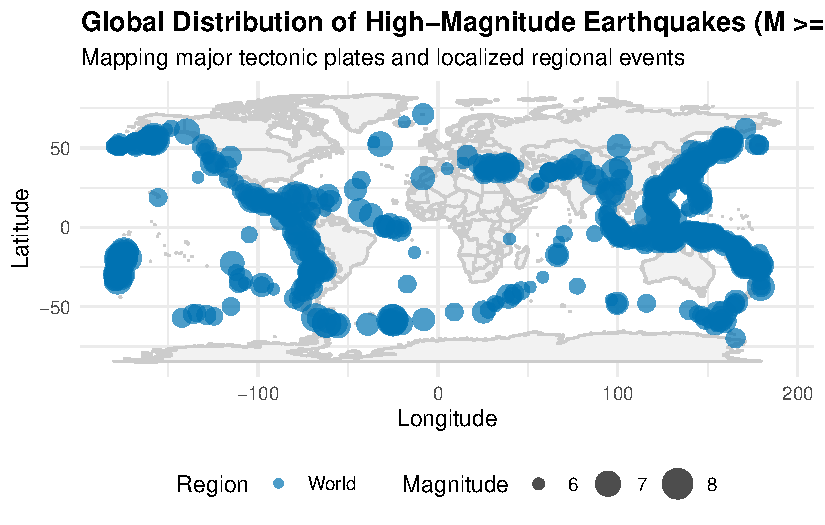
\includegraphics[keepaspectratio]{earthquake_project_files/figure-pdf/unnamed-chunk-5-1.pdf}}

The spatial map underlines that global catastrophic earthquakes are
strongly bound to massive global tectonic plate interfaces, specifically
outlining the Pacific Ring of Fire and the Alp-Himalayan orogenic belt.

Türkiye's high-magnitude events, while less visually expansive on a
world map, are strategically critical because they fall directly atop
densely populated inland zones along the North Anatolian (NAF) and East
Anatolian (EAF) fault lines. This spatial density, combined with the
frequency surge proven by the GLM model, explains why regional risk
monitoring requires unique localized handling rather than reliance on
generalized global baselines.

\section{4. Key Takeaways}\label{key-takeaways}

Topic \& Data Utilized: This study leveraged a comprehensive comparative
framework of 124,701 seismic events spanned across 2020--2026,
integrating local AFAD data with global USGS records to examine
structural risks. Magnitude vs.~Frequency Dynamics: Statistical
visualizations proved that mean earthquake magnitudes remain stable over
time due to fixed physical parameters. True seismic risk variance is
captured via event frequency patterns instead. The Post-2023 Structural
Break: Türkiye experienced a massive structural frequency escalation
after the 2023 Kahramanmaraş events. While global trends remained
completely flat, regional counts surged due to localized plate
adjustments. Advanced Model Validation: A Poisson GLM model
mathematically confirmed that the post-2023 frequency spike in Türkiye
is a highly significant statistical deviation (\(p < 0.001\)),
solidifying the need for separate, regional disaster preparedness
frameworks. Main Outcome: Spatial and quantitative modeling together
prove that global earthquake baselines fail to reflect localized crisis
points. Regional data analytics is an indispensable tool for tailored
infrastructure planning and civil risk allocation.
------------------------------------------------------------------------

\subsubsection{Data Download}\label{data-download}

You can download the unified analytical datasets and the chronological
raw files below:

\begin{itemize}
\tightlist
\item
  \href{data/deprem_verisi.RData}{📥 Download Localized Türkiye Data
  (deprem\_verisi.RData)} --- \emph{Contains filtered regional
  historical points (\(M > 2.0\)).}
\end{itemize}

\paragraph{🌐 Raw Global Records (USGS
Chronology)}\label{raw-global-records-usgs-chronology}

\begin{itemize}
\tightlist
\item
  \href{data/usgs_2020.csv}{📄 Download Raw USGS 2020 Dataset
  (usgs\_2020.csv)}
\item
  \href{data/usgs_2021.csv}{📄 Download Raw USGS 2021 Dataset
  (usgs\_2021.csv)}
\item
  \href{data/usgs_2022.csv}{📄 Download Raw USGS 2022 Dataset
  (usgs\_2022.csv)}
\item
  \href{data/usgs_2023.csv}{📄 Download Raw USGS 2023 Dataset
  (usgs\_2023.csv)}
\item
  \href{data/usgs_2024.csv}{📄 Download Raw USGS 2024 Dataset
  (usgs\_2024.csv)}
\item
  \href{data/usgs_2025.csv}{📄 Download Raw USGS 2025 Dataset
  (usgs\_2025.csv)}
\item
  \href{data/usgs_2026.csv}{📄 Download Raw USGS 2026 Dataset
  (usgs\_2026.csv)}
\end{itemize}




\end{document}
